\begin{figure}[H]
\centering
\shorthandoff{<>}
\begin{tikzpicture}[x=1.45cm,y=3.1cm,font=\small,>=latex]
  \foreach \level in {0.5,1,1.5}{
    \draw[black!10] (0,\level) -- (8,\level);
    \node[left] at (0,\level) {$\level$};
  }
  \fill[teal!12] (1,0) -- plot[domain=1:8,samples=160,variable=\fluxvalue]
    ({\fluxvalue},{1.5*pow(\fluxvalue,-2.5)}) -- (8,0) -- cycle;
  \draw[->,black!65] (0,0) -- (8.6,0);
  \node[anchor=north east] at (8.6,-0.15) {$v=f/F_{\min}$};
  \draw[->,black!65] (0,0) -- (0,1.9) node[above right] {$p_V(v)=F_{\min}\,h_F(F_{\min}v)$};
  \draw[teal!75!black,very thick] (0,0) -- (1,0);
  \draw[teal!75!black,very thick] plot[domain=1:8,samples=160,variable=\fluxvalue]
    ({\fluxvalue},{1.5*pow(\fluxvalue,-2.5)});
  \draw[dashed,black!40] (1,0) -- (1,1.5);
  \fill[teal!75!black] (1,1.5) circle (2.3pt);
  \draw[teal!75!black,fill=white] (1,0) circle (2.3pt);
  \draw[dashed,orange!85!black,thick] (3,0) -- (3,1.08);
  \node[above,align=center,text=orange!75!black] at (3,1.08) {Media: $E[V]=3$\\$E[F]=3F_{\min}$};
  \node[text=teal!75!black] at (5.8,1.5) {$p_V(v)=\dfrac{3}{2}v^{-5/2}$};
  \node[align=center] at (6,0.75) {La cola continúa hasta $+\infty$;\\no hay flujo máximo finito.};
  \draw[->,teal!65!black] (6.6,0.52) -- (7.4,0.04);
  \foreach \tick in {1,2,3,4,5,6,7,8}{
    \draw (\tick,0) -- (\tick,-0.025) node[below] {$\tick$};
  }
  \node[below left] at (0,0) {$0$};
\end{tikzpicture}
\shorthandon{<>}
\caption{Densidad del flujo en la escala $V=F/F_{\min}$, con $F_{\min}=L/(4\pi r_{\max}^2)$. La densidad es cero para $v<1$ y decrece para $v\ge1$: los flujos grandes corresponden a estrellas cercanas al observador y son poco frecuentes. Se muestra sólo hasta $v=8$; el área bajo la curva completa, hasta infinito, es $1$. La línea naranja indica la media, no un límite del flujo.}
\label{fig:densidad-flujo-estelar}
\end{figure}